% !TEX root = m2go1_weik.tex
%==============================================================================
% short introduction to get template running on WINDOWS
% further explanation can be found in the pptx
% can be removed after first compilation 
%
% install MikTeX (http://www.miktex.org) - activate auto-install of packages
% install ActivePerl (https://www.perl.org/) - add to HOME
% system reboot
%
% use command-line or IDE in admin-mode to execute the  following commands
% in the specified order (pdflatex used because we want the PDF in the end)
% 
%
% After changes in glossary you need to execute the following command 
% to use the new acronyms
%
% makeglossaries ma_mustermann
%
% After changes in literature you need to execute the following command
% to use the new reference
%
% bibtex ma_mustermann
%
%==============================================================================


%==============================================================================
% Dokument einrichten und Pakete laden
%==============================================================================

\documentclass[
	pdftex,				% PDFTex verwenden da ausschliesslich ein PDF erzeugt wird.
	a4paper, twoside,	% Verwenden von DIN A4 Papier.
	11pt,				% Grosse Schrift, besser geeignet für A4.
	parskip=half,		% Halbe Zeile Abstand zwischen Absätzen.
	numbers=noenddot,	% Keine Punkte hinter Nummern
	pagesize,           % Schreibt die Papiergroesse in die Datei 
	BCOR=10mm,			% Bindekorrektur
	DIV=13,				% Alternativ 12 oder 14
	headinclude,		% Kopfzeile in den Textbereich
	headsepline,		% Linie nach Kopfzeile.
	openany,            % Keine leere Seite nach/vor neuem Kapitel
	titlepage,
	headings=small,
	bibliography=totocnumbered,	% Bibliographie im TOC nummeriert
]{scrbook}

\usepackage{setspace}\setstretch{1.2} 
%\usepackage{titlesec}

%\titlespacing\section{0pt}{12pt plus 4pt minus 2pt}{0pt plus 2pt minus 2pt}
%\titlespacing\subsection{0pt}{12pt plus 4pt minus 2pt}{0pt plus 2pt minus 2pt}
%\titlespacing\subsubsection{0pt}{12pt plus 4pt minus 2pt}{0pt plus 2pt minus 2pt}

%\usepackage{scrhack}

\usepackage[printonlyused]{acronym}
\usepackage{multicol}

%
% Zeichenkodieruung und Sprache
%

\usepackage[utf8]{inputenc} % Dokument
\usepackage[T1]{fontenc} % Schrift
\usepackage[ngerman, english]{babel}

%
% PDF-Metadaten setzen
%

\usepackage{pdfpages}
\usepackage[
	% Titel des PDF Dokuments
	pdftitle={m2go1_weik},
	% Autor des PDF Dokuments
	pdfauthor={Felix Weik},
	% Thema des PDF Dokuments
	pdfsubject={m2go1_weik},
	% Erzeuger des PDF Dokuments
	pdfcreator={Felix Weik},
	% Schlüsselwörter für das PDF
	pdfkeywords={microservice, web_development, golang, cm, m2go},
	% Dokumenttitel statt Dateiname anzeigen
	pdfdisplaydoctitle=true,																% Sprache des Dokuments
	pdflang=de,
	bookmarksopen=true,
	bookmarksdepth=1,
	colorlinks,
	linkcolor = black,
	citecolor=black,
	urlcolor=black,
]{hyperref}

%
%  Zusätzliche Pakete laden
%

% Anführungszeichen
\usepackage[style=american]{csquotes}

% erweiterte Tabelleneigenschaftn
\usepackage{array, ragged2e}

% Einbinden von Grafiken
\usepackage{graphicx}	

% mathematischer Textsatz
%\usepackage{amsmath}
%\usepackage{amssymb}
%\usepackage{dsfont}

% Textteile drehen
%\usepackage{rotating}	

% Farbpakete
%\usepackage{color}
%\usepackage{xcolor}

% Quellcode sauber formatieren
\usepackage{listings}	

% Font 'Latin Modern Family' verwenden
\usepackage{microtype}
\usepackage{helvet}
\usepackage{mathptmx}

%==============================================================================
% Einstellungen und Definitionen
%==============================================================================

% Farben definieren

\definecolor{light-gray}{gray}{0.95}
%\definecolor{LinkColor}{rgb}{0,0,0.5}
%\definecolor{ListingBackground}{rgb}{0.85,0.85,0.85}
%\definecolor{CommentColor}{rgb}{0, 0.5, 0}
%\definecolor{StringColor}{rgb}{0.63, 0.09, 0.09}

% KOMA-Script Option, Zeilenumbruch bei Bildbeschreibungen.
\setcapindent{1em}

% Stil der Kopf- und Fusszeilen.
\usepackage[headsepline,automark,pagestyleset=KOMA-Script,markcase=ignoreuppercase]{scrlayer-scrpage}
\pagestyle{scrheadings}

% Stil der Überschriften auf normale Schrift.

%\setkomafont{sectioning}{\normalfont\bfseries}		 % Titel mit Normalschrift
\setkomafont{captionlabel}{\normalfont\bfseries}	 % Fette Beschriftungen 
%\setkomafont{pageheadfoot}{\normalfont\itshape}     % Kursive Seitentitel
\setkomafont{descriptionlabel}{\normalfont\bfseries} % Fette Beschreibungstitel

% Codelisting korrekt bezeichnet ausgeben
%\renewcommand\lstlistingname{Source Code}

%==============================================================================
% Listings
%==============================================================================

\lstloadlanguages{% Check Dokumentation for further languages ...
  XML,
  HTML,
  Java,
  Tex
}


\lstset{
  %basicstyle=\scriptsize\ttfamily, % Standardschrift
	basicstyle=\footnotesize\ttfamily,
  %numbers=left, % Ort der Zeilennummern
  %numberstyle=\tiny, % Stil der Zeilennummern
  %stepnumber=2, % Abstand zwischen den Zeilennummern
	%numberblanklines=false,
  numbersep=5pt, % Abstand der Nummern zum Text
  tabsize=2, % Groesse von Tabs
  extendedchars=true, %
  breaklines=true, % Zeilen werden Umgebrochen
  %keywordstyle=\color{red},
  frame=b,
  % keywordstyle=[1]\textbf, % Stil der Keywords
  % keywordstyle=[2]\textbf, %
  % keywordstyle=[3]\textbf, %
  % keywordstyle=[4]\textbf, \sqrt{\sqrt{}} %
  %stringstyle=\color{white}\ttfamily, % Farbe der String
  showspaces=false, % Leerzeichen anzeigen ?
  showtabs=false, % Tabs anzeigen ?
  xleftmargin=17pt,
	xrightmargin=17pt,
  framexleftmargin=17pt,
  framexrightmargin=17pt,
  framexbottommargin=4pt,
  backgroundcolor=\color{white},
  showstringspaces=false % Leerzeichen in Strings anzeigen ?
}

\lstset{literate=%
    {Ö}{{\"O}}1
    {Ä}{{\"A}}1
    {Ü}{{\"U}}1
    {ß}{{\ss}}1
    {ü}{{\"u}}1 
    {ä}{{\"a}}1
    {ö}{{\"o}}1
    {~}{{\textasciitilde}}1
}

\usepackage{caption}
\DeclareCaptionFont{white}{\color{white}}
\DeclareCaptionFormat{listing}{\colorbox[cmyk] {0.43, 0.35, 0.35,0.01}{\parbox{\textwidth-2\fboxsep-2\fboxrule-0pt} {\hspace{15pt}#1#2#3}}}
%\captionsetup[lstlisting]{format=listing,labelfont=bf, textfont=black}

%
% code listing style
%

\lstdefinestyle{kit-cm}{
  backgroundcolor=\color{light-gray},
  belowcaptionskip=1\baselineskip,
  breaklines=true,
  frame=single,
  framexleftmargin=15pt,
  language=C,
  showstringspaces=false,
  basicstyle=\footnotesize\ttfamily, 
  numbers=left,                    
  numbersep=7pt,                
  numberstyle=\tiny\color{black},
  captionpos=b
}

\lstdefinelanguage{Swift}{
  keywords={associatedtype, class, deinit, enum, extension, func, import, init, inout, internal, let, operator, private, protocol, public, static, struct, subscript, typealias, var, break, case, continue, default, defer, do, else, fallthrough, for, guard, if, in, repeat, return, switch, where, while, as, catch, dynamicType, false, is, nil, rethrows, super, self, Self, throw, throws, true, try, associativity, convenience, dynamic, didSet, final, get, infix, indirect, lazy, left, mutating, none, nonmutating, optional, override, postfix, precedence, prefix, Protocol, required, right, set, Type, unowned, weak, willSet},
  ndkeywords={class, export, boolean, throw, implements, import, this},
  sensitive=false,
  comment=[l]{//},
  morecomment=[s]{/*}{*/},
  morestring=[b]',
  morestring=[b]"
}

\lstdefinelanguage{Gherkin}{
	morekeywords = {
		Given,
		When,
		Then,
		And,
		Scenario,
		Feature,
		But,
		Background,
		Scenario Outline,
		Examples
	},
	sensitive=true,
	morecomment=[l]{\#},
	morestring=[b]",
	morestring=[b]'
}

\lstdefinelanguage{json}{
     string=[s]{"}{"},
    stringstyle=\color{blue},
    comment=[l]{:},
    commentstyle=\color{black},
}

\lstdefinelanguage{Golang}{
  morekeywords={break,default,func,interface,select,
  case,defer,go,map,struct,chan,else,goto,package,switch,
  const,fallthrough,if,range,type,continue,for,import,return,var},
  sensitive=true,
  morecomment=[l]{//},
  morecomment=[s]{/*}{*/},
  morestring=[b]",
}

\DeclareCaptionFont{black}{\color{black}} 
\DeclareCaptionFormat{listing}
  {\colorbox{white}
     {\parbox{\dimexpr\textwidth-2\fboxsep}{\centering #1#2#3}}}
\captionsetup[lstlisting]{format=listing,labelfont=bf,textfont=black}

\usepackage{hyperref}
\usepackage{paralist}
\usepackage{subcaption}
\usepackage{booktabs}
\usepackage{listings}
\usepackage{caption}




%
% todo notes
%

\usepackage{todonotes}
%\usepackage[disable]{todonotes}	% hide all todo notes
%\presetkeys{todonotes}{inline}{}	% show all defined todos as inline

%
% glossary
%

%\usepackage[acronym,numberedsection]{glossaries}
%\setacronymstyle{long-short}
%\loadglsentries{chapters/glossar}
%\loadglsentries{chapters/glossar.tex}
%\makeglossaries
%\glsdisablehyper
%
% load additional packages
%

\usepackage{calc}
\usepackage{enumitem}
\usepackage{multirow}
\usepackage{mathtools}
\usepackage{enumitem}
\usepackage{amsmath} 
\usepackage{amssymb}
\usepackage{wasysym}
\usepackage{rotating}
\usepackage{pgfplots}
\usepackage{longtable}
\usepackage{algorithm}
\usepackage{algpseudocode}
\usepackage{float}
\usepackage{pdfpages}
\usepackage{threeparttablex}
\usepackage{longtable,lscape}
\usepackage{tablefootnote}
\usetikzlibrary{patterns}
\usepackage{multicol}
\usepackage{bm}
\usepackage{esvect}
%\usepackage{subfigure}
\floatname{algorithm}{Algorithmus}

\makeindex

\usepackage{bera}% optional: just to have a nice mono-spaced font
\usepackage{listings}
\usepackage{xcolor}

\colorlet{punct}{red!60!black}
\definecolor{background}{HTML}{EEEEEE}
\definecolor{delim}{RGB}{20,105,176}
\colorlet{numb}{magenta!60!black}

\usepackage{tabularx}

\usepackage{listingsutf8}
\pgfplotsset{compat=1.16}
\begin{document}

%==============================================================================

\frontmatter
\setcounter{secnumdepth}{3}
\begin{titlepage}
\thispagestyle{empty}
\enlargethispage{2cm}
%\enlargethispage{\baselineskip}

\sffamily
%\centering
\vspace*{-3.2cm}
\hspace*{-0.6cm}

\includegraphics[height=2.14cm]{figures/kit-logo.png}

\begin{addmargin}{2cm}

\vfill

\begin{tabular}{>{\RaggedRight}p{12cm}}
\begin{center}
{\huge Practical Course Thesis}
\end{center}
\\
\begin{center}
{\textbf{\huge Microservice2Go1 (M2Go1)}}
\end{center}
\\  
\\
\\
\\
\\
\\
   
\\
{M2Go Participant: Felix Weik }  \\
{Semester: 5. Bachelor Semester } \\
\\
\\
{Supervising PhDResearcher: Michael Schneider}  \\
{Supervising SeniorStudent: Frederik Ullrich Klose}  \\
\end{tabular}
\vfill
\vfill
\vfill



%\singlespacing

\vspace{1em}
\begin{tabular}{ll}
	

	Winter Semester 2023 / 2024 \\
	\\
	\multicolumn{2}{l}{Cooperation \& Management (C\&M, Prof. Abeck)} \\
	\multicolumn{2}{l}{Institute for Telematics, Department of Informatics} \\
	\multicolumn{2}{l}{www.cm.tm.kit.edu} \\
	\\
	\multicolumn{2}{l}{\scriptsize{KIT - The Research University in the Helmholtz Association}}\\
\end{tabular}

\end{addmargin}
\newpage
\thispagestyle{empty}
\end{titlepage}
\tableofcontents


\mainmatter
%\glsresetall

\chapter{M2Go Part 1: C\&M Org}
\label{cha:cm_org}

\section{Exercise OnboardingCompletion}
This section contains the answers to the questions of the exercise "OnboardingCompletion".

The first introduction describes the author's motivation for choosing this module.
The second section, the description of the time sheet, explains the author's understanding of the time sheet and its importance.

\subsection{Write an Introduction}
While working as a student intern at Capgemini, I had the opportunity to work in web development for six months.
During this time, I was an integral part of a dynamic team dedicated to an internal project focused on managing events and training programs for their employees.
It was during this time that I discovered the importance of web development and found myself genuinely passionate about the subject.

This exposure gave me a fundamental understanding of web development's potential.
I am thrilled to have chosen this specific module for further education. 
Furthermore, I am eager to explore the possibilities web development offers and look forward to the next few months.

\begin{figure}[H]
    \centering
    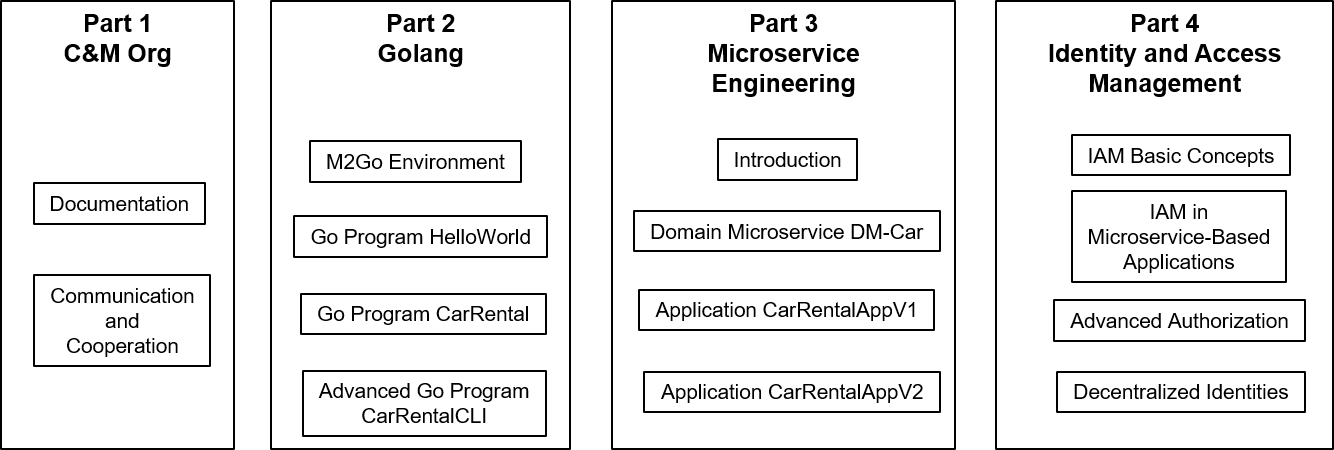
\includegraphics[width=0.8\textwidth]{figures/m2go_parts.png}
    \caption{M2Go Parts}
    \label{fig:m2go_parts}
\end{figure}

\subsection{Describe the Time Sheet}
The time sheet offers a certain overview of the time spent on the project. 
Furthermore, one can compare themselves to the set standards of the project, therefore enabling better time management.
After understanding the provided interface, I was able to fill out the timesheet without any problems.

It helps me and my colleagues build a more structured daily routine and therefore increase productivity. Possible roadblocks or challenges can be identified and solved more easily.
Also, it helps the project manager to keep track of the progress and to identify possible problems, maybe provide assistance if needed.

In essence, the timesheet contributes to streamlined project management and increased, more structured productivity for both individual contributors and project leaders.
\chapter{M2Go Part 2: Golang}
\label{cha:golang}
The first section explains the installation process of the go-environment.
The second section describes the usage and the structure of the GitLab repository.
The third section contains the basic Hello World program and its execution.

Section two is based on the CarRental app and its use cases.

%==============================================================================

\label{sec:exercise_install_go_env}

\subsection{Exercise M2GoEnvironmentInstallation}
\label{sec:exercise_m2go_environment_installation}

\subsubsection*{Environment Description}
The hardware used is a Windows Surface Studio with an 11th Gen Intel Core i5-11300H, 16 GB of RAM, and 256 GB of SSD storage.
The operating system is Windows 11 64-bit. However, the installation is carried out on WSL 2 running Ubuntu 20.04.6 LTS installed on the machine.

\subsubsection*{Installation Steps}
WSL2 (Ubuntu 20.04.6 LTS), VSCode (1.84.2) and Git (2.25.1) are already installed on the machine. 
Therefore no further installation steps are required for these tools.
The correct environment-installation on the author's machine can be seen in \autoref{fig:screendump_installation}.

Carrying out the installation of Go, version go1.21.4 is installed.
To install Go on the machine, the following steps are required:
\begin{enumerate}
    \item Download the latest version of Go from \url{https://go.dev/dl/go1.21.4.linux-386.tar.gz} by using  \texttt{wget} in the terminal.
    \item Extract the downloaded archive to \texttt{/usr/local} via \texttt{sudo tar -C /usr/local -xzf go1.21.3.linux-386.tar.gz}
    \item Under \texttt{/etc/profile} add the following lines to the bottom of the file: 
    \begin{itemize}
        \item \texttt{export PATH=\$PATH:/usr/local/go/bin}
        \item export \texttt{GOPATH=\$HOME/go}
    \end{itemize}
    \item Now reload the terminal or force the update by running \texttt{source \$HOME/.profile}
    \item Verify the installation by running \texttt{go version}
\end{enumerate}

\begin{figure}[H]
	\centering
	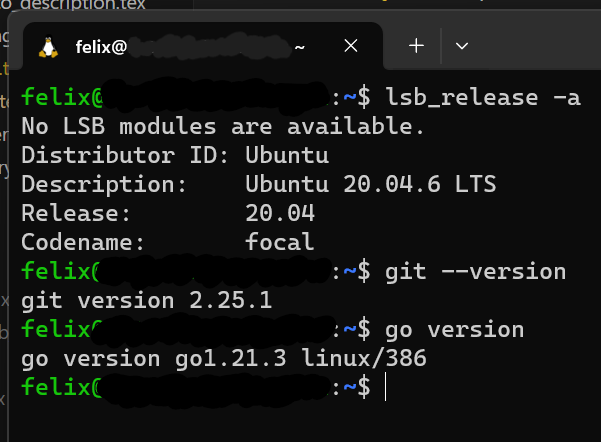
\includegraphics[width=0.5\textwidth]{figures/goLang/installation_screendump.png}
	\caption{Screendump showing the correct installation of the environment}
	\label{fig:screendump_installation}
\end{figure}

Further details on the installation and especially the path variables can be found in \autoref{sec:go_environment_variables} on path variables in Ubuntu.
\label{sec:exercise_cm_gitlab_usage}

\subsection{Exercise CMGitLabUsage}

\subsubsection*{Description of the M2Go Subgroup Structure}
The subgroup structure in \autoref{fig:screendump_subgroupStructure} only contains the Golang repository.
As the course advances, more repositories will be added to this subgroup.
This repository consists of the following three folders:
\begin{enumerate}
    \item BasicGoProgram/HelloWorld: This folder contains the hello world program introducing the basic Golang syntax
    \item CarRental: This folder contains the CarRental program introducing general Golang features
    \item CarRentalCLI: This folder contains the CarRentalCLI program implementing a more complex version of the CarRental program
\end{enumerate}
Furthermore, there is the .gitignore file and the README.md file.
This structure can be further examined in \autoref{fig:screendump_subsubgroupStructure}.

\begin{figure}[h]
    \centering
    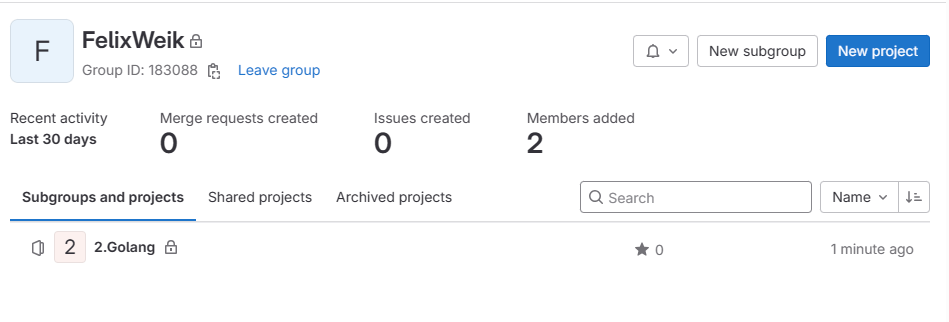
\includegraphics[width=0.8\textwidth]{figures/goLang/golang_personalSubgroupStructure.png}
    \caption{Screendump showing the Subgroup Structure}
    \label{fig:screendump_subgroupStructure}
\end{figure}

\begin{figure}
    \centering
    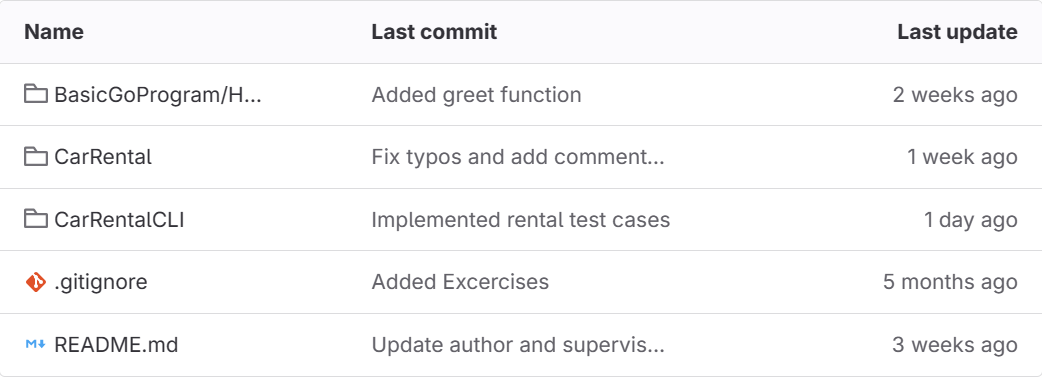
\includegraphics[width=0.8\textwidth]{figures/goLang/golang_personalSubsubgroupStructure.png}
    \caption{Screendump showing the Subgroup Structure of the Golang Folder}
    \label{fig:screendump_subsubgroupStructure}
\end{figure}

\subsubsection*{Repository Cloning Steps}
To clone the repository, the following steps are required:
\begin{enumerate}
    \item Create a Personal Access Token (PAT) on GitLab by going to your Profile Settings and then to Access Tokens
    \item Save the PAT in a safe place
    \item Go to the repository and copy the HTTPS clone URL
    \item Open the WSL2 terminal and navigate to the folder where you want to clone the repository, in the author's case \texttt{/home/felix/WASA\_M2Go}
    \item Download the repository by running the following command in the terminal: \texttt{git clone <HTTPS clone URL>}
\end{enumerate}

\subsubsection*{First Commit}
After changing the placeholder text in the README.md file, the first commit is done by using the graphical features Visual Studio Code offers.
The commit message shown in \autoref{fig:screendump_readmeCommitMessage} is the following: \texttt{Update author and supervisor in README.md}.

After committing the changes, the changes are pushed to the remote repository, which then becomes visible as shown in \autoref{fig:screendump_readme}.

\begin{figure}
    \centering
    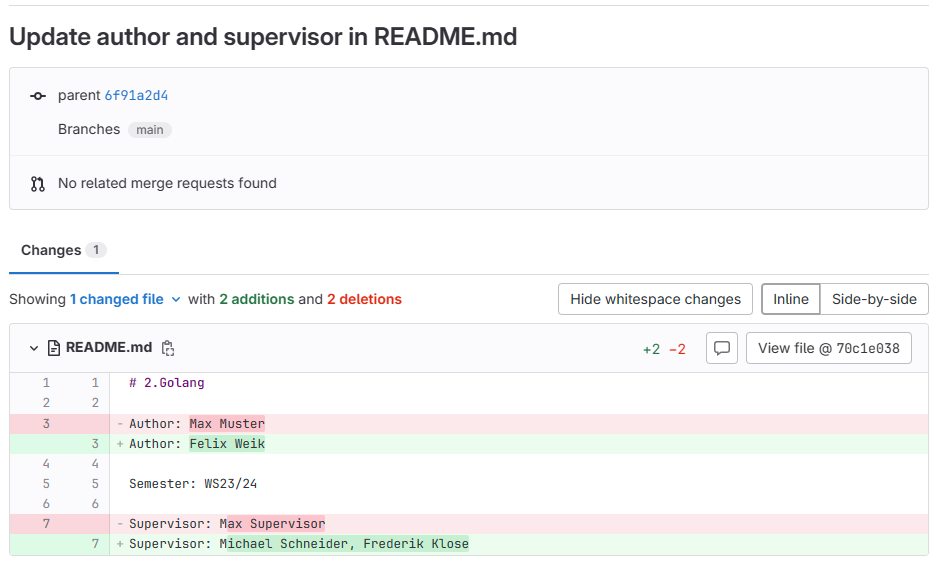
\includegraphics[width=0.8\textwidth]{figures/goLang/golang_screendumpReadmeCommit.png}
    \caption{Screendump showing the Commit Message and the changed Files}
    \label{fig:screendump_readmeCommitMessage}
\end{figure}

\begin{figure}
    \centering
    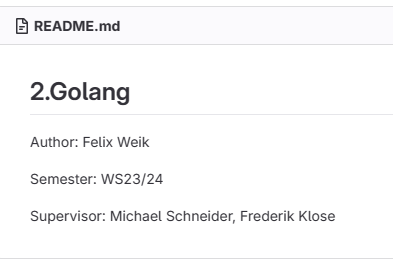
\includegraphics[width=0.5\textwidth]{figures/goLang/golang_screendumpReadme.png}
    \caption{Screendump showing the Updated README.md File}
    \label{fig:screendump_readme}
\end{figure}

\subsection{Excercise HelloWorld}
\label{sec:excercise_hello_world}
% //TODO Einleitung schreiben
% //TODO Listings style updaten 
\subsubsection*{Run Hello World}
After following the instruction in \cite{MS-GODEV}, the code is executed by running \texttt{go run main.go} in the terminal.
The code was executed twice: The first time the given code was executed leading to the output shown in \autoref{fig:screendump_helloWorld_basicExecution}.
The second time the code was executed with different text, which can be seen in \autoref{fig:screendump_helloWorld_differentText}.

\begin{figure}[H]
    \centering
    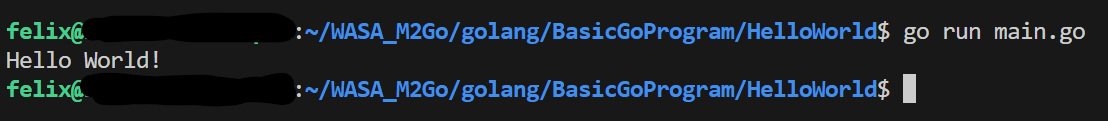
\includegraphics[width=0.8\textwidth]{figures/goLang/helloWorld/golang_helloWorld_basicExecution.png}
    \caption{Screendump showing the basic execution of the Hello World program}
    \label{fig:screendump_helloWorld_basicExecution}
\end{figure}

\begin{figure}[H]
    \centering
    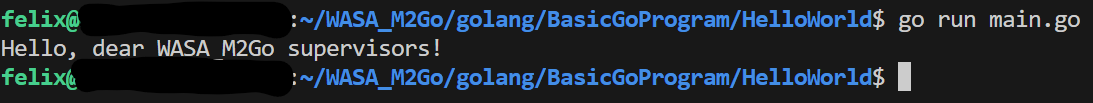
\includegraphics[width=0.8\textwidth]{figures/goLang/helloWorld/golang_helloWorld_ExecutionDifferentText.png}
    \caption{Screendump showing the execution of the Hello World program with different text}
    \label{fig:screendump_helloWorld_differentText}
\end{figure}

\subsubsection*{Code Explanation}
\autoref{lst:helloWorld} shows the code of the Hello World program with explanations of the different parts of the code.
\begin{lstlisting}[
style=kit-cm,
language=Golang,
caption={Hello World Program in Golang with Explanations},
label={lst:helloWorld},
]
// main.go 
// Author: Felix Weik

package main    // package declaration: every executable belongs to the main package
                // by declaring this package, a executable file is produced after compliation

import "fmt"    // import the fmt package, a standard library package 
                // implementing formatted I/O functions
                // after import, one can use the functions of the imported package

func main() {   // declares the function main, which is the 
                // entry point of the program
    fmt.Println("Hello, World!")    // call the Println function 
                                    // of the fmt package; Println prints 
                                    // the given text to the standard output
}               // end of the main function

\end{lstlisting}

\subsubsection*{HelloName}
The goal of this task is to extend the already given HelloWorld program to the HelloName program, prompting the user for a name then showing the given prompt in the output.
The code is shown in \autoref{lst:helloName}:
\begin{lstlisting}[
style=kit-cm,
language=Golang,
caption={Extension of helloWorld to helloName},
label={lst:helloName},
]
// main.go
// Author: Felix Weik

package main

import (
    "fmt"
)

func main() {
    greet()
}

func greet() {
    var name string
    fmt.Print("What is your name? ")
    fmt.Scanln(&name)
    fmt.Println("Hello, " + name + "!")
} 
\end{lstlisting}

The result of the executed code is shown in \autoref{fig:screendump_helloName}

\begin{figure}[H]
    \centering
    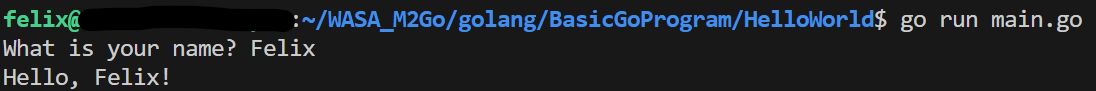
\includegraphics[width=0.8\textwidth]{figures/goLang/helloWorld/golang_helloWorld_helloName.png}
    \caption{Screendump showing the execution of the HelloName program}
    \label{fig:screendump_helloName}
\end{figure}

%==============================================================================

\subsection{Excercise UseCaseDiagram CarRental}
\label{sec:exercise_use_case_diagram_car_rental}
The general functionality of the application CarRental is outlined by Alice's Car Rental story as described in \cite{CM-T-GO} listing 3.1.
It provides a general overview of the application and the user flow of registering and renting a car.

By using the story, the use cases and actors can be derived.
The following tasks are based on the story and help derive the use cases, actors and services modeled in the use case diagram.

\subsubsection*{Derive Use Cases and Actors}
The goal of this task is to find four use cases and one actor according to the given story "Alice's Car Rental" from listing 3.1 in \cite{CM-T-GO}.

% //TODO: Herleitung der vier Use Cases beschreiben
\autoref{lst:car_rental_use_case_1} was derived from line 4 of the given story.

In the story Alice rents a car, a VW ID.2, for a certain period.
This is done by entering the rental period and choosing the car from the list of available cars.

After successfully renting the car, the customer is prompted with a rental confirmation and the rental is stored.

\begin{lstlisting}[
    caption={Use Case 1: "Rent a Car"},
    label={lst:car_rental_use_case_1},
    style=kit-cm,
]
Title: Rent a Car
Primary Actor: Customer
Secondary Actor: None

Preconditions:
    - Customer is registered and logged in
    - Customer has a valid driver's license and credit card

Postconditions:
    - Customer has rented a car for the chosen time interval

Flow:
1. The customer calls the application CarRental.
2. The customer enters a start date and end date as the rental period
3. The system shows a list of the cars that are available at the selected rental period
4. The customer selects one of the listed cars
5. The system shows a rental confirmation and stores the rental

Alternative flows:
3a. no cars are available at the selected time interval
    3a1. The system shows a message that no cars are available at the selected time interval and the flow continues from 2 or terminates
4a. The customer does not want to rent any of the offered cars
    4a1. The flow terminates    
\end{lstlisting}

\autoref{lst:car_rental_use_case_2} describes the registration process itself.

It was derived from line 3 of the given story.
In order to use the application, Alice needs to register first.

After successfully registering, Alice can log in to the application and rent a car.

\begin{lstlisting}[
    caption={Use Case 2: "Registering Process"},
    label={lst:car_rental_use_case_2},
    style=kit-cm,
]
Title: Registering Process
Primary Actor: Customer
Secondary Actor: None

Preconditions:
    - The customer is not registered yet
    - Customer has a valid email address
    - Customer has a valid credit card and driver's license
    - Customer is at least 18 years old
    - Customer is not blacklisted by the car rental company or an insurance company

Postconditions:
    - Customer is registered
    - Customer can rent a car
    - Customer can log in to the car rental company's website

Flow:
1. Customer visits the car rental company's website or opens the app 
2. Customer is asked to register or login
3. Customer clicks on "Register"
4. Customer is prompted for email, name, driver's license, credit card number, date of birth
5. A data validation is performed
6. Customer needs to authenticate his email address
7. Customer chooses a password and a username
8. Customer shows a registration confirmation and the customer is registered successfully 

Alternative flows:
3a. Customer is already registered and clicks on "Login" instead of "Register"
5a. Customer prompts false information or leaves nonoptional fields empty, so the data validation fails
    5a1. The customer is asked to fill out the form again
6a. Customer does not authenticate his email address
    6a1. The customer will not be registered and the registration process will be aborted
7a. Customer chooses a username that is already taken
    7a1. The customer is asked to choose another username
7b. The provided password does not fulfill the given criteria
    7b1. The customer is asked to choose a stronger password
\end{lstlisting}

There are two types of cancellation: Cancellation of a rental and cancellation of the registration.
\autoref{lst:car_rental_use_case_3} describes the cancellation of a rental as described in lines 5 and 6 of the given story.

Like Alice in the story, the customer can cancel a rental if he successfully rented a car but does not want to use it anymore.
The customer can cancel the rental as long as the time interval of the rental has not started yet.

After successfully canceling the rental, the customer is prompted with a cancellation confirmation.

\begin{lstlisting}[
    style=kit-cm,
    caption={Use Case 3: "Cancellation of a Rental"},
    label={lst:car_rental_use_case_3},
]
Title: Cancellation of a Rental
Primary Actor: Customer
Secondary Actor: None

Preconditions:
    - Customer has rented a car
    - Customer is logged in
    - The time interval of the rental has not started yet

Postconditions:
    - Customer has cancelled the rental
    - Customer is prompted with a cancellation fee if necessary

Flow:
1. Customer calls the application CarRental
2. Customer clicks on "My Rentals"
3. Customer selects the rental he wants to cancel
4. Customer clicks on "Cancel Rental"
5. Customer is prompted with a cancellation fee if necessary
6. Customer confirms the cancellation
7. Customer is asked to confirm the cancellation again via email
8. Customer confirms the cancellation via email
9. Customer is prompted with a cancellation confirmation

Alternative flows:
3a. Customer has no rentals
    3a1. The system shows a message that the customer has no rentals and the flow terminates
4a. Customer does not want to cancel the rental and the flow terminates
5a. Customer does not want to pay the cancellation fee
    5a1. The flow terminates and the rental is not canceled
8a. Customer does not confirm the cancellation via email
    8a1. The flow terminates and the rental is not canceled
\end{lstlisting}

\autoref{lst:car_rental_use_case_4} describes the cancellation of the registration as described in line 6 of the given story.

In the story, Alice cancels her registration due to personal reasons.
The customer can cancel the registration if he does not want to use the application anymore.

After successfully canceling the registration, the customer is prompted with a cancellation confirmation and can neither log in nor use the application without registering again.

\begin{lstlisting}[
    float=h,
    caption={Use Case 4: "Cancellation of the Registration"},
    label={lst:car_rental_use_case_4},
    style=kit-cm,
]
Title: Cancellation of the Registration
Primary Actor: Customer
Secondary Actor: None

Preconditions:
    - Customer is registered
    - Customer is logged in
    - Customer has no rentals or outstanding payments

Postconditions:
    - Customer is not registered anymore

Flow:
1. Customer calls the application CarRental
2. Customer clicks on "My Account"
3. Customer clicks on "Cancel Registration"
4. Customer confirmes the cancellation
5. Customer is asked to confirm the cancellation again via email
6. Customer confirms the cancellation via email
7. Customer is prompted with a cancellation confirmation

Alternative flows:
3a. Customer has outstanding payments or rentals
    3a1. The system shows a message that the customer has outstanding payments or rentals and the flow terminates
4a. Customer does not want to cancel the registration and the flow terminates
6a. Customer does not confirm the cancellation via email
    6a1. The flow terminates and the registration is not canceled
\end{lstlisting}

\subsection*{Modelling the Use Case Diagram with UMLet}
The installation of the standalone version of UMLet is carried out as follows:
\begin{enumerate}
    \item Download the latest version of UMLet from \url{https://www.umlet.com/changes.htm}
    \item Extract the downloaded archive
    \item Run the executable file \texttt{umlet.sh} in the extracted folder
\end{enumerate}

A screen dump of the folder structure of the extracted archive is shown in \autoref{fig:umlet_folder_structure}.
\begin{figure}
    \centering
    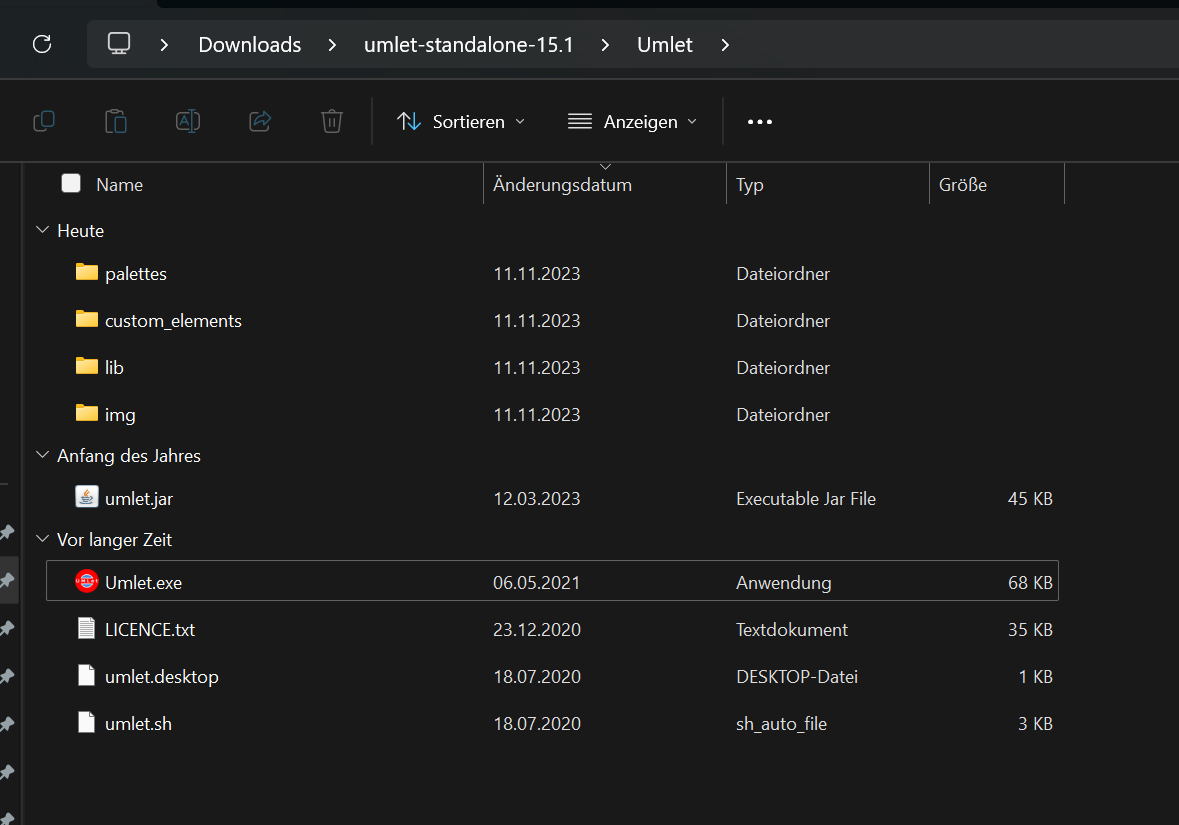
\includegraphics[width=0.8\textwidth]{figures/goLang/carRental/carRental_umletInstallation.png}
    \caption{Folder structure of the extracted UMLet archive}
    \label{fig:umlet_folder_structure}
\end{figure}

The use case diagram is shown in \autoref{fig:car_rental_use_case_diagram}.

It uses so-called services to abstract the implementation of the application.
By providing services, the implementation of the application can be changed without changing the use cases.

The registration service is used to register a customer.
It provides the user interface and structures to interact with the customer.
The registration service itself uses the authentification service to provide the customer with a secure way to authenticate himself, for example by two-factor authentification.
It also uses the cancellation service to cancel the registration if the customer wants to do so.

The rental service is used to rent a car.
It interacts with the location service, providing the location of the customer and the cars and displaying it on a map.
It also uses the cancellation service to cancel the rental if the customer wants to do so.
The car usage service is used to provide the customer with information about the car, for example, if the car is available, the current fuel level or the current mileage.

The services' interactions are displayed in the use case diagram utilizing the arrows and the corresponding labels.
\begin{figure}[H]
    \centering
    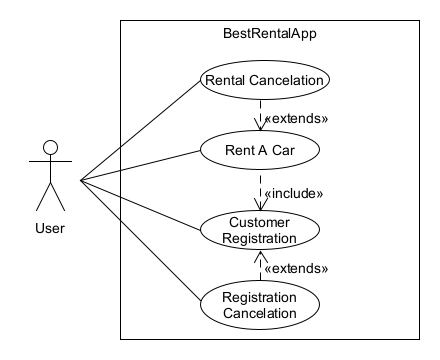
\includegraphics[width=0.8\textwidth]{figures/goLang/carRental/carRental_umlDiagram.png}
    \caption{Use case diagram of the car rental application}
    \label{fig:car_rental_use_case_diagram}
\end{figure}

\subsection{Excercise UseCase RentACar}
\label{sec:exercise_use_case_rent_a_car}
\subsubsection*{Alice's Car Rental}
This task aims to complete the use-case story "Rent a Car" for Alice.
This is done by adding the given data from the story to the use-case story.

The completed use-case story is shown in \autoref{lst:alices_car_rental_use_case_1}.

\begin{lstlisting}[
style=kit-cm,
caption={Alice's Version of Use Case 1},
label={lst:alices_car_rental_use_case_1},
]
1. Alice calls the application CarRental.
2. Alice enters 01.01.00 as a start date and 02.02.00 as the end date as the rental period
3. The system shows a list of the cars that are available at the selected rental period
4. Alice selects a VW ID.2
5. The system shows a rental confirmation and stores the rental

Alternative flows:
3a. The VW ID.2 is not available at the selected time interval
    3a1. The system shows a message that the VW ID.2 is not available at the selected time interval and the flow continues from step 2 or terminates
4a. Alice does not want to rent the VW ID.2
    4a1. The flow terminates
\end{lstlisting}

\label{cha:design_of_data_and_functionality}

\section{Design of the Data and the Functionality}

\subsection{Description of the Initial Entity Diagram}

\subsection{Adding the Attributes}

\subsection{Adding the Functionality as a Method}

\section{Excercise CarRentalStructs}
\label{sec:car_rental_structs}

\subsection*{Add the Attributes to Structs}
After adding the attributes from the entity diagram to the 
\texttt{.../golang/CarRental/CarRentalStructs/CarRentalStructs.go} path and saving
the IDE automatically formats the code and indents it correctly.

\subsection*{Initialize and Print Structs}
The result of the initialization and printing of the structs is shown in figure \ref{fig:car_rental_structs}.
\begin{figure}[H]
    \centering
    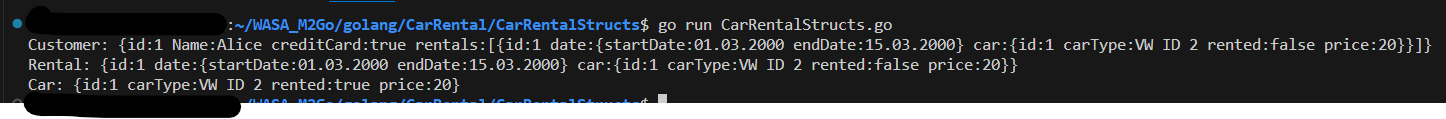
\includegraphics[width=\textwidth]{figures/goLang/carRental/carRental_structs.png}
    \caption{Output of the structs}
    \label{fig:car_rental_structs}
\end{figure}

\subsection*{Create an Array of Rentals}
The function works as follows:
\begin{enumerate}
    \item The array \texttt{cartypes} holds the string of 5 different cartypes
    \item The function \texttt{createRentals(id, date, car)} returns 5 rentals that are appended to the array
    \item Via \texttt{fmt.Println(rentals)} the array is printed into the console
\end{enumerate}

The result looks like this:
\begin{figure}
    \centering
    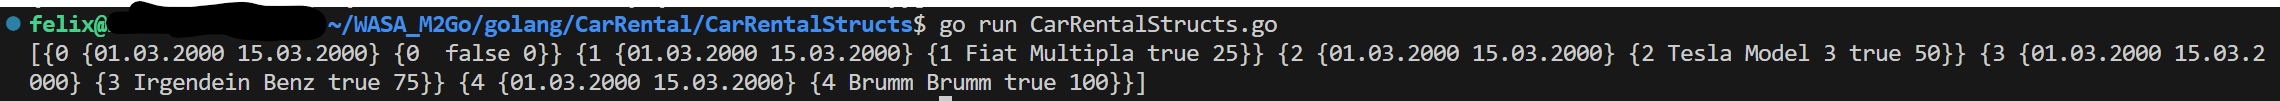
\includegraphics{figures/goLang/carRental/carRental_arrayFiveRentals.png}
    \caption{Output of the Array of Rentals}
    \label{fig:car_rental_array_five_rentals}
\end{figure}


%==============================================================================
%\chapter{M2Go Part 3: Microservice Engineering}
\label{cha:microservice_engineering}
%//TODO: Einleitung für gesammtes Aufgabenkapitel
%====================================================
%//TODO: Aufgaben kurz erläutern
\section{Introduction}
\subsection{Excercise UMEGeneralConcepts}
\label{sec:ume_general_concepts}
%//TODO: Kurze Einleitung
\subsubsection*{Architectural Style}
The Unified Microservice Engineering approach aligns with the microservices architectural style.
This involves breaking down an application into smaller, independent services that can be developed, deployed, and scaled separately.
The services communicate with each other through APIs and are usually organized around business capabilities.
These services aim to enhance flexibility, scalability, and maintainability.

Predecessors of the microservices architectural style are the service-oriented architecture (SOA) and the distributed systems architectural style which will be further explained in the following.

\paragraph*{Service Oriented Architecture}
SOA shares some similarities with the microservices architectural style.
The focus is on organizing services around business capabilities and developing them independently.
This aims to achieve reusability and interoperability.

Yet, microservices tend to be generally smaller, more fine-grained, decoupled and are usually lightweight.

\paragraph*{Distributed Systems}
Distributed systems represent a collection of independent computers, appearing to the users of the system as a single coherent system.
These systems handle tasks across a network, each node having its local memory and set of responsibilities.

Microservices share a similar idea: Splitting an application into smaller, more independent services communicating with each other.
Each microservice manages its functionalities and data to provide the overall functionality of the application.

\subsubsection*{Domain Modelling}
A domain model describes selected aspects of a domain in a conceptual model, yet the model should not separate the concept from the implementation.
This model can be used to better understand the domain and to communicate with stakeholders.

The domain model is located in the domain logic layer of the layered architecture.
Therefore each microservice implements its domain model.

Using a layered software architecture, the business logic layer is separated into application logic and domain logic.
The application logic layer contains the application-specific logic while the domain logic layer contains the domain-specific logic.
This domain-specific logic is derived from the domain model, enabling the domain knowledge to be encapsulated in the domain logic layer.
The application logic layer is derived from the analysis of the application requirements, for instance, use cases.

Therefore the domain logic layer is the part of the software architecture that is shaped the most by domain modeling.

\subsubsection*{Modelling of the Architecture}
To model the architecture of a microservice-based application, UME uses the Unified Modeling Language (UML).
To create the according diagrams, the UMLet tool is used.

Two modeling views can be distinguished: the tactical and the strategic view.

The strategic modeling provides an overview of the domain model.
The result is the so-called context map.
It provides the link to the microservice architecture.
The context map consists of subdomains and their bounded contexts.
A bounded context can be seen as a microservice candidate.

Tactical modeling takes a closer look at the entities and their relationships.
Each bounded context entity models the static relations of the domain entity.

\subsection{Excercise APIStyles}
\label{sec:api_styles}
%//TODO: Kurze Einleitung
\subsubsection*{REST and gRPC}
Representational state Transfer (REST) and Remote Procedure Call (gRPC) are two different frameworks and collections of best practices and technologies for building APIs.

The main conceptual difference is the focus and orientation of both concepts:
REST is resource-oriented.
Each resource has a unique identifier (URI) and can be accessed using the standardized HTTP methods.
Therefore, there is only a small set of well-defined methods for manipulating the resources.
gRPC is procedure, method, or function-oriented.
It is based on the idea of implementing a service, offering remotely callable methods.
These methods can be called by a client with their parameters and return values.

Both concepts have their legitimate use cases, yet it is important to choose the right one for the given use case.

\subsubsection*{REST Properties}
% Name and describe the main properties of the API style REST.
REST provides a concept of how microservices' APIs should be designed.
Its main properties are explained in the following.

\paragraph*{Addressable Ressources:}
As mentioned before, REST is resource-oriented meaning that each resource has a unique identifier, a URL, and can be accessed using the standardized HTTP methods.
Therefore only a small set of functions is needed to manipulate the resources, offering a uniform interface.

\paragraph*{Stateless Communication:}
REST is stateless meaning that each request is independent of the previous one.
The server, therefore, does not need to store any information about the client.
The client must transfer all the information in the request that is needed to process it to the server.
This leads to a loss of performance.
Yet, this is a tradeoff for an increase in scalability and robustness.

\paragraph*{Representation Orientation:}
This principle strongly relates to resources.
These resources have to be represented.
This happens in a standardized format, for instance, JSON or XML.
The client can choose the format that suits him best.
MIME, the Multipurpose Internet Mail Extensions standard, defines the different formats used in internet protocols.

\subsubsection*{gRPC Components}
% Name and describe the main components of the gRPC architecture.

\subsubsection*{Use of REST and gRPC in UME}
% Which API style is appropriate for which type of microservice in the UME approach?

\subsection{Excercise ArchitectureCarRentalAppV1.0}
\label{sec:architecture_car_rental_app_v1_0}
%//TODO: Kurze Einleitung

%====================================================


%\chapter{Summary}
\label{cha:summary_outlook}
This module introduced the UME approach for designing microservices.
Each step, namely the analysis, the design, the implementation and testing as well as the deployment and the operations of different microservice kinds were explained.
This included learning the techniques and tools for each step.
The following paragraphs summarize each part of this practical course thesis.

\begin{description}
    \item[Part 1: C\&M Org] The first part of this module introduced the C\&M organization and the necessary tools for the practical course.
    This included the time sheet, understanding the timesheet and communication processes.
    \item[Part 2: Golang] This part focused on the programming language Go and the correct installation of the development environment.
    The first Go program, Hello World, was implemented introducing basic Go syntax and concepts.
    The second program introduced the analysis phase of the UME approach on the example program \texttt{CarRental}.
    This helped to understand the importance of the analysis artifacts and the analysis phase.
    \texttt{CarRental} was extended with a CLI, making it the \texttt{CarRentalCLI} program.
    First implementation steps were made to implement the missing functionality.
    \item[Part 3: Microservice Engineering] This part introduced the application microservice \texttt{AM-RentalManagement} and the domain microservice \texttt{DM-Car}.
    To fully understand the differences, the API styles \texttt{ReST} and \texttt{gRPC} were introduced.
    Also, different modeling views were distinguished. \\
    \texttt{DM-CarV1.0} was implemented using the \texttt{ReST} API style.
    The API diagram was analyzed leading to the specification of the API endpoints in the OpenAPI specification.
    Text cases were derived from OCL constraints, added to the OpenAPI specification, and implemented using the Go testing framework.
    Additional functionality was implemented to extend the functionality of \texttt{DM-CarV1.0}.
    Finally, the application was containerized using Docker and deployed using Docker Compose. \\
    \texttt{AM-RentalManagementV1.0} was implemented using the \texttt{gRPC} API style.
    Analysis artifacts were analyzed, learning the differences between API diagrams of application and domain microservices.
    Finally, the protobuf specification language was used to specify the API endpoints.
    The challenge of orchestration, the API controller, and local deployment introduced further concepts of microservice engineering.
\end{description}

In summary, this course introduced the UME approach for designing microservices.
Each step was explained in detail, and tools and techniques were introduced and applied.
This does not only equip the students with tools like Go, Docker, and Kubernetes but also with a holistic understanding of microservice engineering through the complete UME approach.

\bibliographystyle{cmnat}
\bibliography{m2go1}

%==============================================================================

\end{document}